%TC第29.1节练习 4、5
%TC第29.2节练习 2、4、6
%TC第29.3节练习 5
%TC第29.4节练习 2
%%%%%%%%%%%%%%%%%%%%%%%%%%%%%%%%%%%%%%%%%%%%%%%%%%%%%%%%%%%%%%%%
\documentclass[11pt, a4paper, UTF8]{ctexart}
%%%%%%%%%%%%%%%%%%%%%%%%%%%%%%%%%%%
% File: preamble.tex
%%%%%%%%%%%%%%%%%%%%%%%%%%%%%%%%%%%

\usepackage[top = 1.5cm]{geometry}

% Set fonts commands
\newcommand{\song}{\CJKfamily{song}} 
\newcommand{\hei}{\CJKfamily{hei}} 
\newcommand{\kai}{\CJKfamily{kai}} 
\newcommand{\fs}{\CJKfamily{fs}}

\newcommand{\me}[2]{\author{{\bfseries 姓名:}\underline{#1}\hspace{2em}{\bfseries 学号:}\underline{#2}}}

% Always keep this.
\newcommand{\noplagiarism}{
  \begin{center}
    \fbox{\begin{tabular}{@{}c@{}}
      请独立完成作业,不得抄袭。\\
      若得到他人帮助, 请致谢。\\
      若参考了其它资料,请给出引用。\\
      鼓励讨论,但需独立书写解题过程。
    \end{tabular}}
  \end{center}
}

% Each hw consists of three parts:
% (1) this homework
\newcommand{\beginthishw}{\part{作业}}
% (2) corrections (Optional)
\newcommand{\begincorrection}{\part{订正}}
% (3) any feedback (Optional)
\newcommand{\beginfb}{\part{反馈}}

% For math
\usepackage{amsmath}
\usepackage{amsfonts}
\usepackage{amssymb}

% Define theorem-like environments
\usepackage[amsmath, thmmarks]{ntheorem}

\theoremstyle{break}
\theorembodyfont{\song}
\theoremseparator{}
\newtheorem*{problem}{题目}


\theoremheaderfont{\kai\bfseries}
\theoremseparator{:}
% \newtheorem*{remark}{注}
\theorempostwork{\bigskip\hrule}
\newtheorem*{solution}{解答}
\theorempostwork{\bigskip\hrule}
\newtheorem*{revision}{订正}

\theoremstyle{plain}
\newtheorem*{cause}{错因分析}
\newtheorem*{remark}{注}

\theoremstyle{break}
\theorempostwork{\bigskip\hrule}
\theoremsymbol{\ensuremath{\Box}}
\newtheorem*{proof}{证明}

\renewcommand\figurename{图}
\renewcommand\tablename{表}

% For figures
% for fig with caption: #1: width/size; #2: fig file; #3: fig caption
\newcommand{\fig}[3]{
  \begin{figure}[htp]
    \centering
      \includegraphics[#1]{#2}
      \caption{#3}
  \end{figure}
}

% for fig without caption: #1: width/size; #2: fig file
\newcommand{\fignocaption}[2]{
  \begin{figure}[htp]
    \centering
    \includegraphics[#1]{#2}
  \end{figure}
}
\usepackage{blindtext}
\usepackage[utf8]{inputenc}
\usepackage{amsmath,bm}
\usepackage{amstext}
\usepackage{amsfonts}
\usepackage{amsmath}
\title{机器学习导论}
\me{殷天润}{171240565}
\date{\today}

\begin{document}
\maketitle
\noplagiarism

%%%%%%%%%%%%%%%%%%%%%%%%%%%%%%%%%%%%%%%%%%%%%%%%%%%%%%%%%%%%%%%%
%                       Homework START!                        %
%%%%%%%%%%%%%%%%%%%%%%%%%%%%%%%%%%%%%%%%%%%%%%%%%%%%%%%%%%%%%%%%
\beginthishw
%%%%%%%%%%%%%%%%%%%%
\begin{problem}[ML problem 1]
\begin{enumerate}
	\item Please give the cumulative distribution function F$_X$(x) for X;
	\item Define random variable Y as Y = 1/($X^2$), please give the proba
	bility density function f$_Y$ (y) for Y ;
	\item A proof problemThe probability distribution of random variable $X$ follows:\\
	\begin{equation}
	f_X(x)=\begin{cases}
	\frac{1}{2} & 0<x<1;\\
	\frac{1}{6} & 2<x<5;\\
	0 & \text{otherwise}.
	\end{cases}
	\end{equation} 
	(1) [5pts] Please give the cumulative distribution function $F_X(x)$ for X;\\ \\ 
	(2) [5pts] Define random variable $Y$ as $Y=1/(X^2)$, please give the probability density function $f_Y(y)$ for $Y$;\\ \\
	(3) [10pts] For some random non-negative random variable Z, please prove the following two formulations are equivalent:\\
	\begin{equation}
	\mathbb{E}[Z]=\int^\infty_{z=0} z f(z)\mathrm{d}z,
	\end{equation}
	\begin{equation}
	\mathbb{E}[Z]=\int^\infty_{z=0} \mathrm{Pr}[Z\geq z]\mathrm{d}z,
	\end{equation}
	Meantime, please calculate the expectation of random variable $X$ and $Y$ by these two expectation formulations to verify your proof.
\end{enumerate}

\end{problem}
\begin{solution}
    \begin{enumerate}
    \item $$ F_{X}(x)=\left\{
    \begin{array}{rcl}
    0       &      & {-\infty <x \leq 0 }\\
    \dfrac{1}{2}x     &      & {0<x\leq 1}\\
    \dfrac{1}{2}     &      & {1<x \leq 2}\\
    \dfrac{1}{6}+\dfrac{1}{6}x       &      & {2<x \leq 5}\\
    1 & & {otherwise.}
    \end{array} \right. $$
    \item $F_{Y}(Y\leq y)=P(\dfrac{1}{x^{2}}\leq y)=P(-\dfrac{1}{\sqrt{y}}\leq x\leq \dfrac{1}{\sqrt{y}})=1-F_{X}(\dfrac{1}{\sqrt{y}})$
    
    Then, $f_{Y}(y)=F\prime _{Y}(y)=\dfrac{1}{2}y^{-\dfrac{3}{2}}P_x(\sqrt{\dfrac{1}{y}})$.
    
    Therefore, $$ f_{Y}(y)=\left\{
    \begin{array}{rcl}
   
    \dfrac{1}{12}y^{-\dfrac{3}{2}}    &      & {\dfrac{1}{25}<y\leq \dfrac{1}{4}}\\

    \dfrac{1}{4}y^{-\dfrac{3}{2}}       &      & {1\leq y < \infty}\\
    0 & & {otherwise.}
    \end{array} \right. $$
	\item 	$\mathbb{E}[X]=\int^\infty_{z=0} \mathrm{Pr}[Z\geq z]\mathrm{d}z=\int^\infty_{z=0}\int^{t=z}_{t=0}1 dt f(z)dz=\int^\infty_{z=0} z f(z)\mathrm{d}z$
	\begin{enumerate}
	\item 
	
	\begin{enumerate}
	\item $\mathbb{E}[X]=\dfrac{1}{2}*(1-0)* \dfrac{1}{2}+\dfrac{1}{2}*(25-4)*\dfrac{1}{6}=\dfrac{1}{4}+\dfrac{7}{4}=2$
	\item $\mathbb{E}[X]=\int^\infty_{x=0} \mathrm{Pr}[X\geq x ]=\int^\infty_{x=0} \mathrm(1-{Pr}[X\leq x])=\int^\infty_{x=0} \mathrm{1-F_X{x}}$
	
	Therefore, $\mathbb{E}[X]=\dfrac{3}{4}+\dfrac{1}{2}+\dfrac{3}{4}=2$
	\end{enumerate}
	\item 
	\begin{enumerate}
	\item $\mathbb{E}[Y]=(\sum k_i)\int^\infty_{z=0}\sqrt{y}=+\infty$($k_i$为某个正的常数,不需要关心)
	\item 注意到$F_{X}(x)=\dfrac{1}{2}x\quad (x\in (0,1]))$,并且$F_{Y}=1-F_{X}(\dfrac{1}{\sqrt{y}})$,所以$F_{Y}$不收敛,$\mathbb{E}[Y]=+\infty$
	\end{enumerate}
\end{enumerate}
\end{enumerate}
    
\end{solution}




\begin{problem}[ML problem 2]
	Let $D\in \mathbb{R}^2$ be a finite set. Define a function $E: \mathbb{R}^3 \rightarrow \mathbb{R}$ by\\
\begin{equation}
E(a,b,c)=\sum\limits_{x\in\mathcal{D}}(ax^2_1+bx_1+c-x_2)^2.
\end{equation}
(1) [10pts] Show that $E$ is convex.\\ \\
(2) [10pts] Does there exist a set $D$ such that $E$ is strongly convex? Proof or a counterexample.
\end{problem}
\begin{solution}
    \begin{enumerate}
    	\item 准备使用黑塞阵来证明;
    	
    $$
    	H_x=\sum\limits_{x_1\in\mathcal{D}}{
    		\left[ \begin{array}{ccc}
    		2*x_{1}^{4} & 2*x_1^{3} & 2*x_1^{2}\\
    		2*x_1^{3} & 2*x_{1}^{2} & 2*x_1\\
    		2*x_1^{2} & 2*x_1 & 2
    		\end{array} 
    		\right ]}, 
    	$$
    	
	特征值:对于求和中的某一个$x_1$,$$|\lambda E-H_x|={
    		\left| \begin{array}{ccc}
    		x_{1}^{4}-\lambda & x_1^{3} & x_1^{2}\\
    		x_1^{3} & x_{1}^{2}-\lambda & x_1\\
    		x_1^{2} & x_1 & 1-\lambda
    		\end{array} 
    		\right |}
	$$
	特征方程为(省略计算步骤):$\lambda^{2}(x^{4}+x^{2}+1-\lambda )=0$,$\lambda_{1}=\lambda_{2}=0,\lambda_{3}=1+x^{2}+x^{4}>0$
	因此黑塞矩阵中作为求和必定大于等于0,黑塞矩阵半正定,E是convex的。
    
    \item 由第一题的作答,黑塞矩阵必有两个为0的特征值,因此它不是正定但是是半正定的,因此不存在
    \end{enumerate}
\end{solution}




\begin{problem}[ML problem 3]
Suppose $x_k$ is the fraction of NJU students who prefer course A at year $k$. The remaining fraction $y_k = 1-x_k$ prefers course B. \\\\
At year $k + 1$, $\frac{1}{5}$ of those who prefer course A change their mind. Also at the same year, $\frac{1}{10}$ of those who prefer course B change their mind (possibly after taking the problem 3 last year). \\ \\ 
Create the matrix P to give $[x_{k+1}\quad y_{k+1}]^\top = P [x_k\quad y_k]^\top$ and find the limit of $P^k[1\quad 0]^\top$ as $k \rightarrow \infty$.
\end{problem}

\begin{solution}
	\begin{enumerate}

		\item $x_{k+1}=-\frac{1}{5}x_{k}+\frac{1}{10}y_{k}$
		,$y_{k+1}=\frac{1}{5}x_k-\frac{1}{10}y_k$

		所以$$
			P={
			\left[ \begin{array}{cc}
			-\frac{1}{5} & \frac{1}{10} \\
			\frac{1}{5} & -\frac{1}{10} 
			\end{array} 
			\right ]},		
		$$
		计算特征值并对角化:$${
			\left[ \begin{array}{cc}
			0 & 1 \\
			0 & -1
			\end{array} 
			\right ]}^{-1}{
			\left[ \begin{array}{cc}
			0 & 0 \\
			0 & -\frac{3}{10} 
			\end{array} 
			\right ]}{
			\left[ \begin{array}{cc}
			0 & 1 \\
			0 & -1
			\end{array} 
			\right ]}$$
		因此$$P^{k}[1\quad 0]^{T}={
			\left[ \begin{array}{cc}
			0 & 1 \\
			0 & -1
			\end{array} 
			\right ]}^{-1}{
			\left[ \begin{array}{cc}
			0 & 0 \\
			0 & (-\frac{3}{10})^{k} 
			\end{array} 
			\right ]}{
			\left[ \begin{array}{cc}
			0 & 1 \\
			0 & -1
			\end{array} 
			\right ]}{
			\left[ \begin{array}{c}
			1  \\
			0 
			\end{array} 
			\right ]}$$
		当k$\rightarrow \infty$的时候,上面的式子趋向于0
	
	\end{enumerate}
    
\end{solution}




\begin{problem}[ML problem 4]
Yesterday, a student was caught by the teacher when tossing a coin in class. The teacher is very nice and did not want to make things difficult. S(he) wished the student to determine \emph{if the coin is biased for heads} with $\alpha = 0.05$.\\ \\
Also, according to the student’s desk mate, the coin was tossed for $50$ times and it got $35$ heads. \\ \\
(1) [10pts] Show all calculate and rules (hint: using z-test). \\ \\
(2) [10pts] Calculate the p-value and interpret it.
\end{problem}
\begin{solution}
    \begin{enumerate}
    	\item 假设:$$H_0: \mu_0=0.5$$
    	
    	因为$\alpha =0.05$,查表得到$\mu_{\dfrac{\alpha}{2}}=1.96$;
    	
    	数据量较小,我在excel里面手动用$\sigma=\sqrt{\dfrac{1}{n+1}*\sum (x_i-0.5)^{2}}$的公式算到了$\sigma $约为0.505076
    	
    	计算:
    	$$|\dfrac{\bar{X}-\mu_0}{\sigma / \sqrt{n}}|=|\dfrac{0.7-0.5}{0.505076272
    	/7.071067811865
    }|\thickapprox 2.8>1.96$$

所以落在了拒绝域,不太可能发生。(这硬币应该不均匀)
\item p-value=P$\{Z\geq 2.80\}$$\thickapprox 1-0.9974=0.0026$;

这意味着硬币均匀重量的概率大约是0.0026,概率非常小
    \end{enumerate}
\end{solution}





\begin{problem}[ML problem 5]

	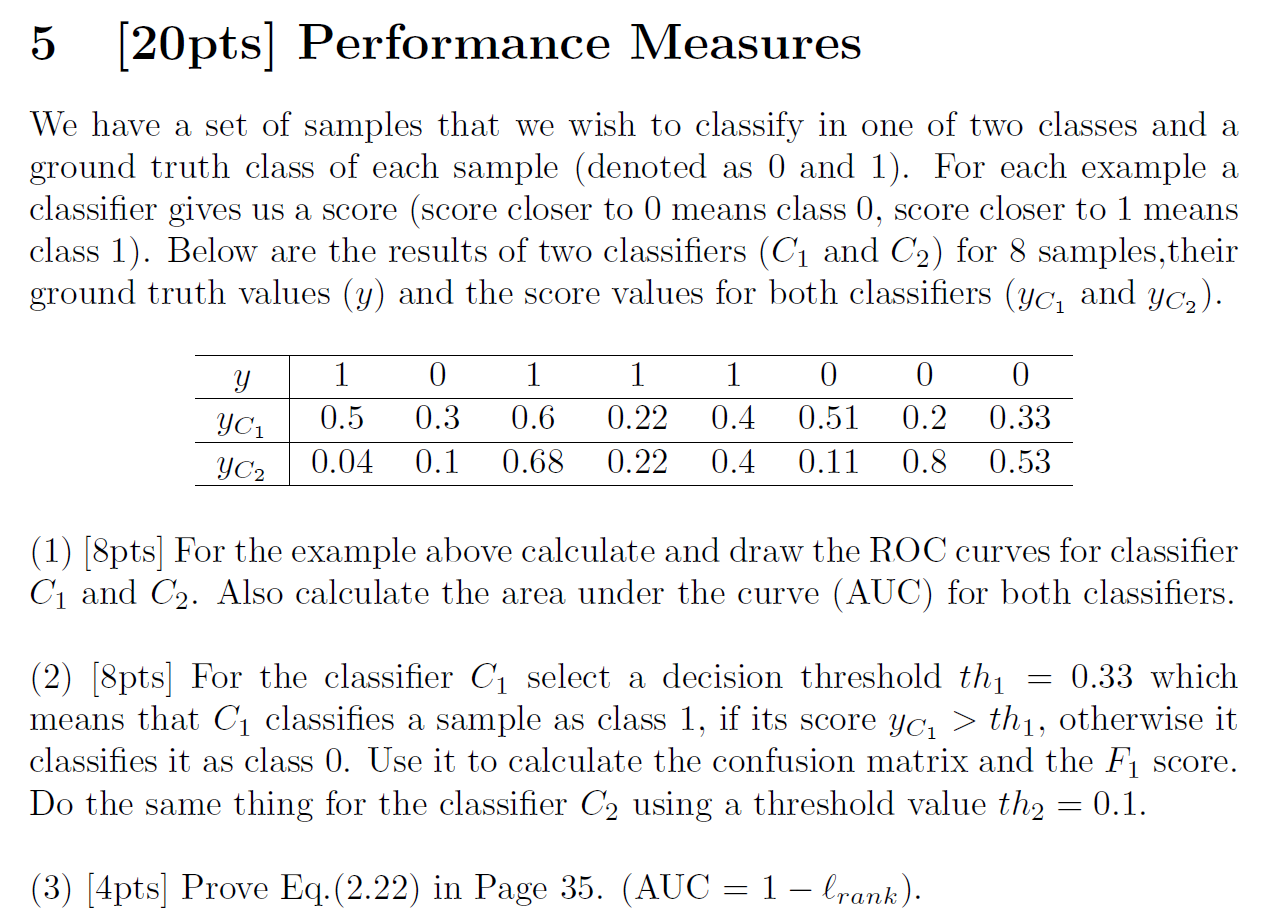
\includegraphics[scale=0.3]{5-p.png}

\end{problem}
\newpage
\begin{solution}
    \begin{enumerate}
    	\item 我用python的sklearn库做了ROC曲线,纵轴是TPR,横轴是FPR,如下面的图
    	
    	\begin{figure}[h]
    		
    		\centering
    	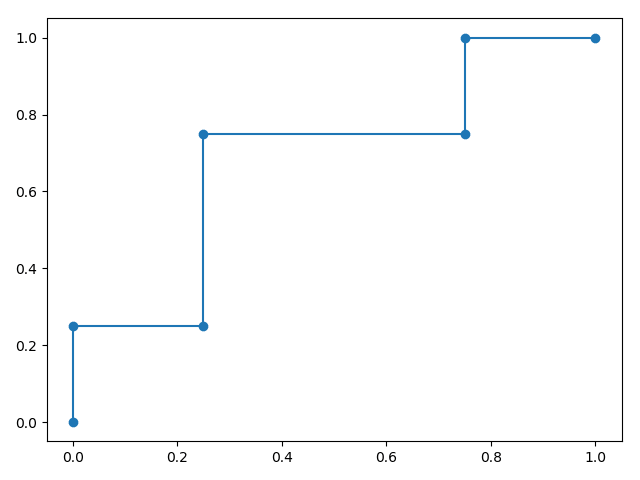
\includegraphics[scale=0.3]{5-C1.png}
    	\caption{ROC figure of C1}
    	\end{figure}
    	\begin{figure}[h]
    	
    	\centering
    	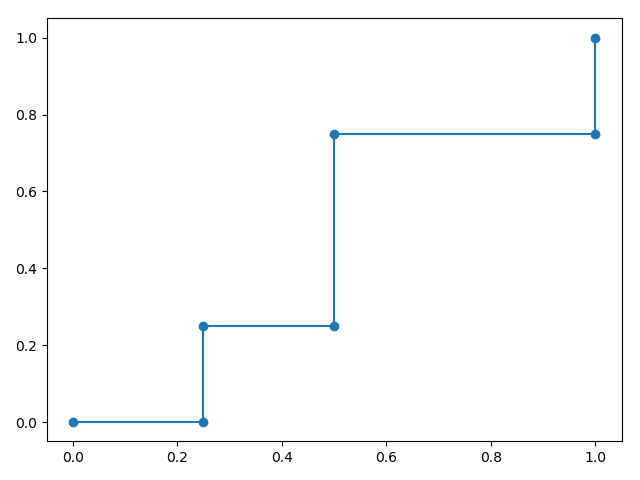
\includegraphics[scale=0.3]{5-C2.png}
    	\caption{ROC figure of C2}
    	
    	其中,C1的AUC的值为0.6875,C2的AUC值为0.4375
    \end{figure}
\item 
C1的 混淆矩阵
$$\begin{pmatrix}
3 & 1 \\
1 & 3
\end{pmatrix}$$
$$P=3/(3+1)=0.75,R=3/(3+3)=0.5;$$
$$F1=2*0.75*0.5/(0.75+0.5)=0.6;$$
C2的混淆矩阵
$$\begin{pmatrix}
2 & 2 \\
2 & 2
\end{pmatrix}$$
$$P=2/(2+2)=0.5,R=2/(2+2)=0.5;$$
$$F1=2*0.5*0.5/(0.5+0.5)=0.5$$
    \end{enumerate}
\end{solution}





\begin{problem}[TC 29.4-2]
	For least squares linear regression problem, we assume our linear model as:\\
\begin{equation}
y=x^T \beta+\epsilon,
\end{equation}
where $\epsilon$ is noise and follows $\epsilon\sim N(0,\sigma^2)$. Note the instance feature of training data $\mathcal{D}$ as $\bm{X}\in\mathbb{R}^{p\times m}$ and note the label as $\bm{Y}\in\mathbb{R}^n$, where $n$ is the number of instance and $p$ is the feature dimension. So the estimation of model parameter is:\\
\begin{equation}
\hat{\beta}=(\bm{XX}^T)^{-1}\bm{XY}.
\end{equation}
For some given test instance $x_0$, please proof the expected prediction error $\text{\bf{EPE}}(x_0)$ follows:\\
\begin{equation}
\text{\bf{EPE}}(x_0)=\sigma^2+\mathbb{E}_{\mathcal{D}}[x^T_0(\bm{XX}^T)^{-1} x_0\sigma^2].
\end{equation}
Please give the steps and details of your proof.(Hint: $\text{\bf{EPE}}(x_0)=\mathbb{E}_{y_0|x_0}\mathbb{E}_{\mathcal{D}}[(y_0-\hat{y}_0)^2]$, you can also refer to the proof progress of variance-bias decomposition on the page 45 of our reference book)
\end{problem}
\begin{solution}
    
\end{solution}
%%%%%%%%%%%%%%%%%%%%%%%%%%%%%%%%%%%%%%%%%%%%%%%%%%%%%%%%%%%%%%%%
%                      Correction START!                       %
%%%%%%%%%%%%%%%%%%%%%%%%%%%%%%%%%%%%%%%%%%%%%%%%%%%%%%%%%%%%%%%%
%\begincorrection
%%%%%%%%%%%%%%%%%%%%
%\begin{problem}[]

%\end{problem}

%\begin{cause}
%
%\end{cause}

%\begin{revision}

%\end{revision}
%%%%%%%%%%%%%%%%%%%%
%\newpage
%%%%%%%%%%%%%%%%%%%%





%%%%%%%%%%%%%%%%%%%%%%%%%%%%%%%%%%%%%%%%%%%%%%%%%%%%%%%%%%%%%%%%
%                       Feedback START!                        %
%%%%%%%%%%%%%%%%%%%%%%%%%%%%%%%%%%%%%%%%%%%%%%%%%%%%%%%%%%%%%%%%
%\beginfb
%\begin{itemize}
%
%\end{itemize}





%%%%%%%%%%%%%%%%%%%%%%%%%%%%%%%%%%%%%%%%%%%%%%%%%%%%%%%%%%%%%%%%
%                        Homework END!                         %
%%%%%%%%%%%%%%%%%%%%%%%%%%%%%%%%%%%%%%%%%%%%%%%%%%%%%%%%%%%%%%%%
\end{document}
